%*****************************************
\chapter{Implementation}
\label{ch:implementation}
%*****************************************

%\hint{This chapter should describe the details of the implementation addressing the following questions: \\ \\
%1. What are the design decisions made? \\
%2. What is the environment the approach is developed in? \\
%3. How are components mapped to classes of the source code? \\
%4. How do the components interact with each other?  \\
%5. What are limitations of the implementation? \\ \\
%The section should have a length of about five pages.}

Up to this point, the presented information is on a conceptual level. In contrast, this chapter examines the actual implementation in our framework.\footnote{We make our source code openly available in a public GitHub repository.\\ https://github.com/TimUnverzagt/Thesis}

\section{Representation of the components}
Chapter \ref{ch:design} defines an experiment by its architecture, training parameters, and pruning setup. Figure \ref{fig:Setup Representation} clarifies where those components can be found in the framework. 
Additionally, figure \ref{fig:Dataset Representation} describes which datasets are available. If we preprocessed a dataset, it notes the location of the responsible code.\\
The natural language dataset, Reuters-21578, consists of legacy code that was not used in any of the presented experiments. It was implemented during the search of a topic for this thesis.
\begin{figure}
	\centering
	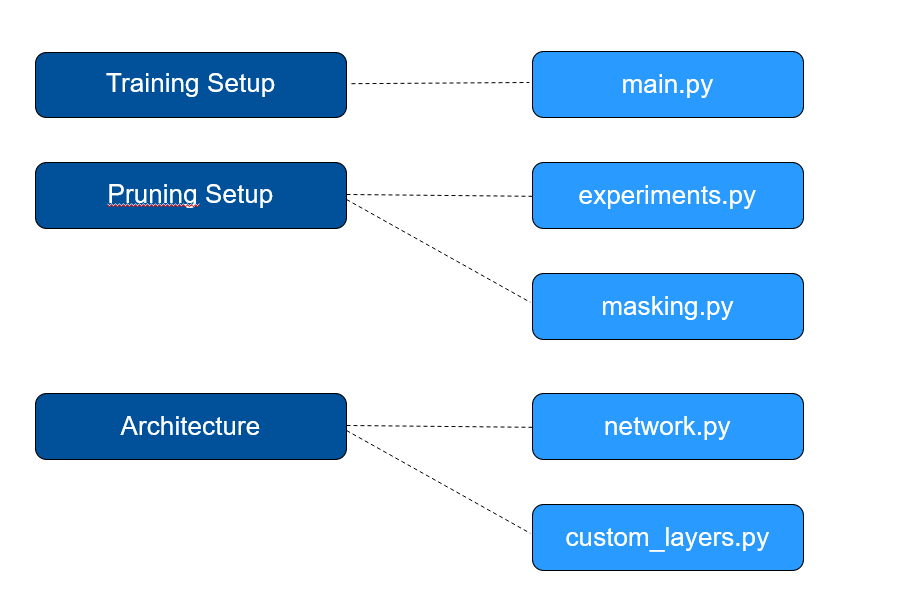
\includegraphics[width=400px]{gfx/5-Implementation/setups.png}
	\caption{Representation of the main components in the framework}
	\label{fig:Setup Representation}
	\vspace{7pt}
	\footnotesize{
		Source:\\
		This figure was produced by the author.
	}
\end{figure}
\begin{figure}
	\centering
	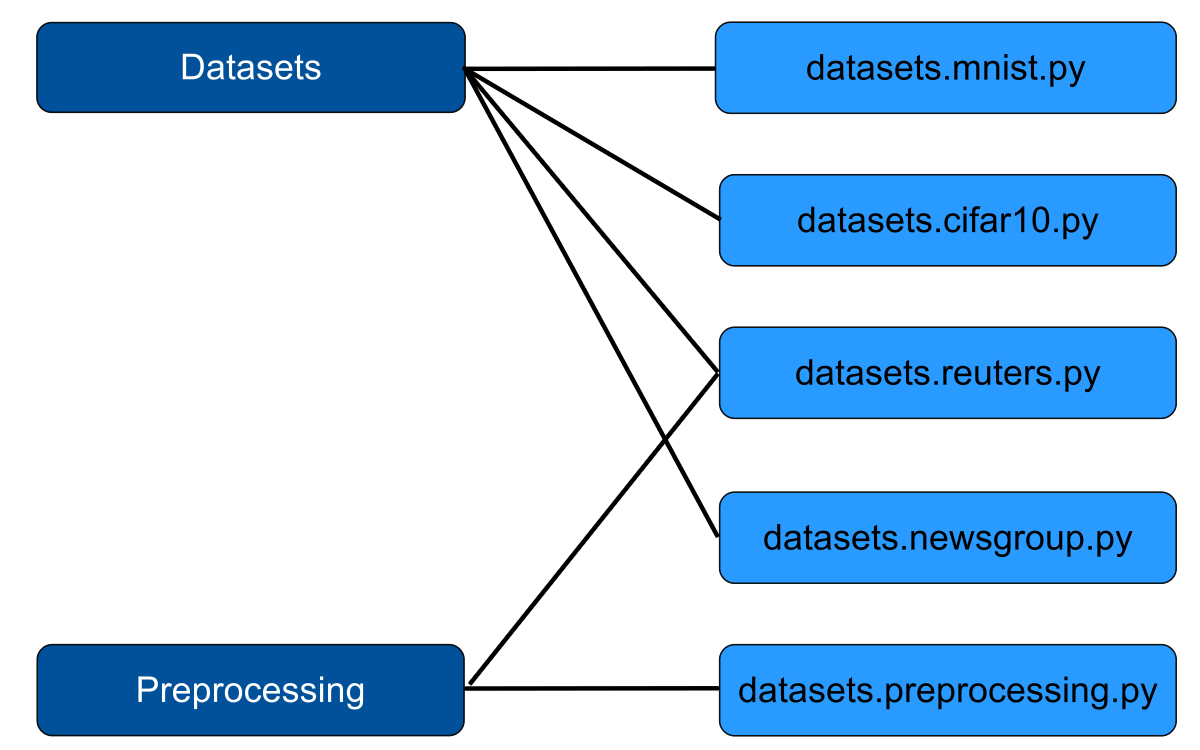
\includegraphics[width=400px]{gfx/5-Implementation/datasets.png}
	\caption{Representation of the datasets and their preprocessing in the framework}
	\label{fig:Dataset Representation}
	\vspace{7pt}
	\footnotesize{
		Source:\\
		This figure was produced by the author.
	}
\end{figure}

%\begin{figure}
%	\begin{minipage}{0.45\textwidth}
%	\end{minipage}\hfill
%	\begin{minipage}{0.45\textwidth}
%	\end{minipage}
%\end{figure} 

\section{Execution Flow}
The framework differentiates three layers of abstraction. Any single module should only ever use data on the same level of abstraction.
The highest layer defines the training setup, chooses parameters for the remaining layers, collects the resulting training histories, and saves them. Optionally the results can be visualized, either directly or from saved files. 
On the next layer, the framework loads the dataset and instantiates the network wrapper. Afterward, it trains the network while collecting metrics into histories, and prunes it when appropriate.
The lowest layer of the framework forms the interface to the neural network backend. Here, architectures are implemented, models are trained, and weights are masked to model the pruning of connections.
Figure \ref{fig:Example Control Flow} depicts a scheme of the framework during one of the experiments. The highlighted pieces define the particular execution flow.
\begin{figure}
	\centering
	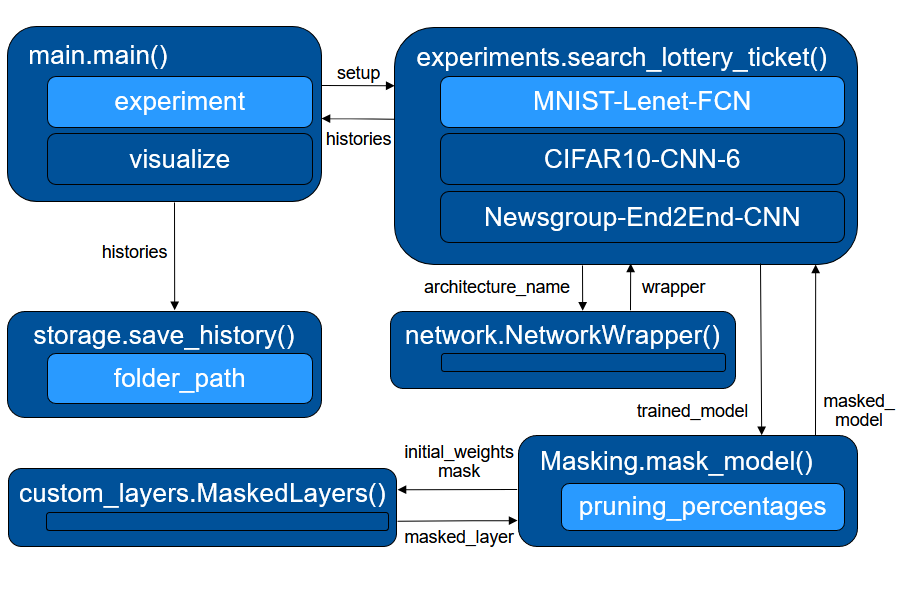
\includegraphics[width=400px]{gfx/5-Implementation/control_flow.png}
	\caption{Scheme of the framework during an example experiment}
	\label{fig:Example Control Flow}
	\vspace{7pt}
	\footnotesize{
		Source:\\
		This figure was produced by the author.
	}
\end{figure}

%-----

\section{Backend}

\subsection{Networks}
\textbf{Tensorflow 2.0} supplies a functional API capable of implementing all networks described in this thesis and many more. It also distributes training to devices other than regulars CPU cores.\cite{Tensorflow} Of particular interest to this work is the speed-up achieved through the usage of GPUs.
Because Tensorflow did not correctly handle the utilized multiclass data during the calculation of network accuracy, we also adopted, \textbf{scikit-learn}, an additional machine learning package for the on-line evaluation. 
Scikit-learn is an open-source python framework built on \textit{NumPy}, \textit{SciPy}, and \textit{matplotlib} that supplies a plethora of data analysis tools.\cite{scikit-learn}

\subsection{Datasets and Preprocessing}
The framework retrieves the datasets MNIST and CIFAR10 from a Tensorflow interface. The corresponding modules of the supplied framework read out these interfaces, bring the data into the expected shape, and return the canonical split of training and test data points. 
For the 20Newsgroups dataset, the framework utilizes a scikit-interface.\\
We employ the Word Tokenizer of \textbf{NLTK}, an open-source natural language framework that also contains the Reuters-21578 dataset.\cite{NLTK}

\subsection{I/O-Elements}
The supplied framework employs the object-serialization package \textbf{pickle} to save the history of an experiment directly. This type of storage is meant \textbf{for internal use only}. On their website, the packages authors explicitly warn of untrusted data that was saved with pickle.

\section{Limitations}
While our codebase is generally capable of unraveling and reproducing any architecture described in the functional Tensorflow API, it only supports the masking of the layers described in chapter \ref{ch:design} so far. Additionally, Tensorflow itself does not support the pruning of single neural connections because they are bundled together in the tensors used to model layers. As it can only flag whole tensors as non-trainable, a different solution is necessary. Our framework utilizes the same workaround recorded by J. Frankle and M. Carbin and represents pruned weights through masks on the layers tensors.
